\chapter{Discussion} \label{ch5:discussion}
% Ska egentligen inte heta discussion.
This chapter concludes the thesis. Initially the research questions are addressed, before the results are evaluated in the context of the implementation. Finally, a section providing guidance for any future work is included.

\section{Research Questions}

The Research Questions initially introduced in Chapter \ref{ch1:introduction} are discussed in the following subsections.

\subsection{Handling Arbitrary Shapes}\label{subsec:ArbiShapes}

The biggest difference between the \gls{SQ} and \gls{GJK} when it comes to the ability to deal with arbitrary shapes of obstacles is related to that of convexity.

The \gls{GJK} relies on the points being arranged in a convex shape. Minkowski summing convex shapes will result in another convex shape, and conversely any concavity will also be transferred onward into the resulting shape, within which the algorithm tries to find the origin.

Consider, in 2D, a case where the Minkowski difference returns a \textbf{C}-shaped figure with the origin located in between the tips but outside of the figure. In such a case it would be trivial to pick three points in the C and construct a triangle encapsulating the origin, but it would not provide any information regarding whether the origin is actually on the C or not. Contrast this to a case with the \textbf{D}-shaped figure, with the origin in the center.

For \gls{SQ} however, checking whether a point is in a non-convex is as simple as checking whether a point is in a convex \gls{SQ}. Thus, there are whole families of shapes that \gls{SQ} can represent better than what could be done with \gls{GJK}.

\begin{figure}[h]
	\centering
	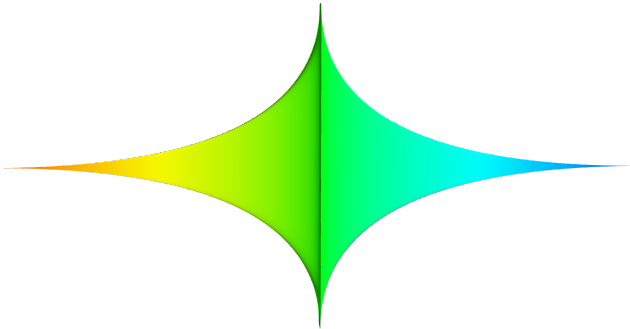
\includegraphics[width=0.5\textwidth]{import/SQ_Concave}
	\caption{Non-convex: $a_1=0.5$, $a_2=5$, $a_3=10$, $\epsilon_1=4$, $\epsilon_2=0.2$. }
	\label{fig:SQ_ConcaveLink}
\end{figure} 

Figure \ref{fig:SQ_ConcaveLink} shows one non-convex link that the \gls{GJK} algorithm would not be able to properly handle as is. One would have to artificially inflate the shape and make the pinched sides straight to have it work with \gls{GJK}.

\begin{figure}[h]
	\centering
	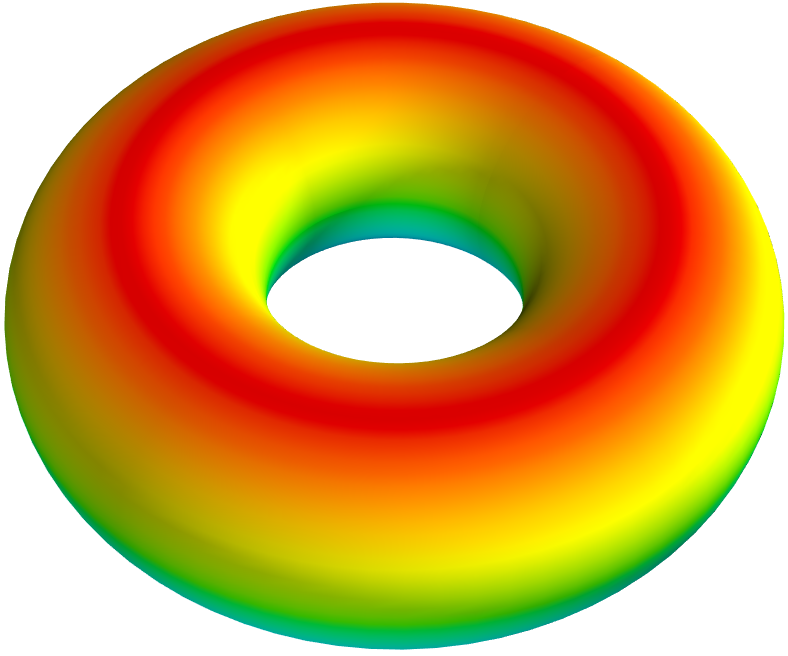
\includegraphics[width=0.35\textwidth]{import/SQ_Toroid}
	\caption{Supertoroid: $a_1=2$, $a_2=2$, $a_3=1$, $\epsilon_1=1$, $\epsilon_2=1$. }
	\label{fig:SQ_Toroid}
\end{figure} 

Figure \ref{fig:SQ_Toroid} shows a supertoroid, a non-convex shape that the \gls{GJK} algorithm would require be broken up into several convex primitives (e.g., overlapping spheres) to then do the check separately for each. A trade off would have to be made between amount of computations and accuracy. For fewer computations, bigger and fewer pieces would need to be used, sacrificing accuracy. More, smaller pieces could better follow the true shape of the supertoroid but would obviously require more computation.

While it is outside the scope of this work, it is worth restating the fact that \gls{SQ} can be further manipulated and deformed using the taper, bend and twist operations mentioned in Section \ref{subsubsec:SQDeform}.  

Finally, in defense of the \gls{GJK} algorithm, the creation of (convexly clustered) points for it to use will always be much more straightforward. To create a \gls{SQ} it has to either be manually created by tuning the dimension and shape parameters, or by solving an optimization problem to fit it to the points.


\subsection{Modeling a 6 DoF Arm}

The ability to be able to model arbitrary shapes and being able to conveniently do collision detection on them is useful. The discourse in Section \ref{subsec:ArbiShapes} regarding the arbitrary shapes of obstacles applies here as well. The supertoroid, for example, is very useful for modeling a ring-shaped \gls{EE} part of a robotic manipulator. The bending operation, though not part of this work, allows for creating links that are inherently curved with a non-convexity.

In practice, to increase fitting accuracy multiple objects (\gls{SQ} or general polytopes) have to be used, combining primitives into a a more complex whole. \gls{SQ} make for very customizable primitives, which in return means even better fitting modeling. \gls{GJK} and polytopes will always be simpler to set up, though they might require more sets of polytope clouds to compensate for the same non-convex overall structure.	


\subsection{Qualitative Analysis of A*}

The qualitative analysis of the A* algorithm is presented here.

\subsubsection{Memory Issues}
A*, when used in motion planning, means finding a path in configuration space. Assuming that the space is divided into hypercube units with orthogonal sides, a 2D hypercube (a square) has four sides into which the algorithm can expand; and a 3D hypercube (a cube) has six faces. Extrapolating, any $n$-dimensional hypercube will have $2n$ corresponding hypercubes the algorithm can expand into.

Thus, as the number of \gls{DoF} increase, the memory space required to hold the graph nodes also increases dramatically. This can result in significant problems, if not a total collapse of the algorithm and the computing unit it is running on. The \gls{RRT} algorithm does not suffer from this problem with higher \gls{DoF}.

One way to remedy this would be to reduce the resolution parameter such that each hypercube occupies a bigger volume, reducing the total number of hypercubes. The advantage of a robotic manipulator having many \gls{DoF} is precisely that the redundancy of the joints increases the probability that a feasible path will be found. Thus, it is conceivable that A* could be successfully used for motion planning high \gls{DoF} manipulators, with the resolution parameter set low to compensate. Of course, then setting the resolution parameter (and parameter tuning in general) becomes another issue for the engineer to deal with. Regarding this specific topic, more research is required to fully be able to answer.

\subsubsection{Parameter Tuning}

A* is resolution complete and relies on having properly tuned parameters to even be able to find a solution (if one exists). This can be difficult to know beforehand. Even then, as previously mentioned, an increased resolution will increase the memory requirements and will also lead to an increased computation time.

\gls{RRT} is probabilistically complete, and will return a solution (provided that it exists) given enough time. However, it is not bereft of the need to manually tune some parameters. The difference is that it will not affect its ability to return a solution, just its ability to do it in a reasonable time frame. The parameter in question is the maximum distance $d$, which limits how far away from the tree a new node in configuration space can be located. A very small $d$ will result in many nodes having to be generated to explore the same amount of space. But a very large $d$ will result in a very long line segment that needs to be checked for collisions. 

In the \gls{RRT} implementation of this thesis, it is possible to set a maximum distance (defined as Euclidean distance in configuration space between radian angle values) as well as a second parameter: interval number. The default is ten, such that it will collision check the old node, the new node and the eight angle configurations between them. If the combination of these two parameters in the implementation is not thorough enough, the algorithm could be at risk of approving a line segment between two angle configurations that in reality has a collision. 

A* does come with a small risk of producing false negative collision checks. The biggest danger lies in specific critical regions, like the boundary between free space and the forbidden region. One simple way to mitigate this risk is to insert a safety margin around the forbidden region of at least one hypercube, as false positives are slightly more preferable over false negatives, even at the risk of not being able to return valid paths.

\subsubsection{Forbidden Regions}

One of the stated benefits of using \gls{RRT} is that it allows for the forbidden configuration space to be calculated \textit{ad hoc}, when it is necessary, and not \textit{a priori} for the whole space.

For A*, the algorithm itself is generally agnostic to this, provided that a heuristic function is not used that requires the a priori explicit computation of the forbidden regions. For example a heuristics measure of "distance to closest forbidden region" would necessitate this kind of calculation, though it is not clear if such a heuristic would be considered admissible for use in A* in the first place. 

\subsection{Evaluation of the Computational Memory Management}

From a memory standpoint, the \gls{GJK} algorithm needs explicit representations of all objects, both links and objects. The \gls{SQ} algorithms on the other hand only requires an explicit representation of one of them; for the one that is implicitly represented, only the five $a_*$ and $\epsilon_*$, as well as six translation and rotation parameters need to be stored. These are a negligible number compared to $n^2$. As such, \gls{GJK} keeps $O(n^2 \times (l + o))$ points in memory, and \gls{SQ} keeps either $O(n^2 \times o)$ or $O(n^2 \times l)$ in memory.


\subsection{Evaluation of the Computational Processing Time}
 
\subsubsection{Regarding the Implementation}

Since the collision detection methods were implemented as black box methods, the \gls{RRT} acted as a multiplicative factor on each algorithm's respective computation time. Considering that creating motion plans for a six \gls{DoF} arm required hours of processing time, one of the first conclusions to make is that the implementation was slow. This can most likely be attributed to the fact that it was written in Python, a dynamically typed, interpreted high-level language. Typically, if this had been used in a production environment like in a simulation engine or on a robot the algorithms would have been written in a compiled language like C or C++. However, as these issues are shared by both algorithm implementations they do not affect the difference in relative performance between them.




\subsubsection{Comparison}

When there were no collisions (i.e. the tests from Sections \ref{subsec:Test1}, \ref{subsec:Test3}, \ref{subsec:Test4}), there was surprisingly not much of a difference in performance between the algorithms, even when dramatically varying the number of links, obstacles or even points $n^2$. The Reverse-\gls{SQ} generally outdid the Obverse-\gls{SQ}, perhaps due to small fixed costs associated with jumping between loops in the implementation. 

This lack of difference in performance can most likely be attributed to the support mapping function of the \gls{GJK}, which is also composed of a for loop looping through the points to find the most extreme point. It runs this function twice (for $K_A$ and $K_B$, in lieu of taking the Minkowski sum and then performing it on $K_C$). If there is no collision, the algorithm will in the second iteration fail to find a point on the other side of the origin, terminating in accordance with Termination Condition 1 and returning a false. Thus, it has had to sweep through $2 \times n^2$ points twice to conclude a non-collision. It is also possible that the algorithm managed to set up a $2$-simplex (line), with the edges on each side of the origin, but then be unable to find a third point on the other side of the origin, resulting in the algorithm having swept through $2 \times n^2$ three times. Finally, the worst case is if it draws up a $3$-simplex (triangle) but terminates when it fails to find a fourth point. Since the initial search vector is randomly initialized, the algorithm can produce different execution times for the same collision detection scenario.

The \gls{SQ} algorithms, however, sweep through $n^2$ points of one object and calculate the $F(.)$ inside-outside implicit function of the other object for each point. This calculation is only done once for each point, and as the $n^2$ points are only looped through once for each check, it is advantageous in comparison to the support mapping function even if the individual calculations might take a longer time themselves. Furthermore, when there is a collision, unless the \gls{GJK} algorithm specifically returns the origin itself (Termination Condition 2), the \gls{GJK} algorithm is doomed to either do four iterations of its algorithm (Termination Condition 3), or to get stuck in a non-stopping loop, hit $i_{max}$ and trigger Termination Condition 4. All of these will require more point sweeps, which increase the computational work. 

This would explain the results of the test rounds in Section \ref{subsec:Test2}, where the \gls{GJK} algorithm was outclassed by the \gls{SQ} algorithms, going by the average times listed in Section \ref{subsec:Test2}.

It is also evident that the \gls{GJK} is a more sensitive algorithm. In the case where it terminated in accordance with Termination Condition 4 in Section \ref{subsec:Test2}, it took 1.275 seconds, roughly five times as long as it should have taken. This is quite an extraordinary long time and can be attributed to the $i_{max}$ being too high and most likely needing to be lowered. This was not experimented with, as it was considered too specific to the \gls{GJK} algorithm and only came into  effect in rare cases.

In some specific cases where collision has taken place, the \gls{SQ} algorithm(s) have the ability to immediately return a collision. For example, in Test 2.I the R\gls{SQ} returns a collision answer incredibly fast at 0.0007 seconds. This is because the algorithms loops through the arm links and check each with the obstacle, beginning with the base (Link 0). As the R\gls{SQ} checks whether each point is within the obstacle or not, and the points are very tightly concentrated, the algorithm almost immediately returns a collision. The O\gls{SQ} algorithm must however loop through the points of the sphere until it reaches the "latitude" at which the sphere intersects with the base. 

Note that there is a potential to miss a collision here, if one \gls{SQ} object is much smaller than the other \gls{SQ} and if it has fully entered the other, the algorithm which explicitly represents the bigger object and implicitly the smaller object will miss a collision as only the surface is explicitly represented. The mirror \gls{SQ} collision detection algorithm will of course be able to detect this collision. In practice, this is very unlikely to happen as the \gls{RRT} algorithm checks collisions between angle configurations by incrementing the links forward. It is similar to the case when $n$ is too small and point density is lost, as mentioned in Section \ref{subsec:SQIntersect}.

Regarding the \gls{RRT}, the inherent random nature of the vanilla \gls{RRT} algorithm makes it impossible to judge if a specific combination of \gls{RRT} and collision detection algorithms is superior. The \gls{GJK} generally had lower execution times than both R\gls{SQ} and O\gls{SQ}, producing the absolute fastest execution time at 148 seconds in \gls{RRT} Test V. This does however not mean much, as it cannot be attributed to some conceived superior quality of \gls{GJK}, as opposed to random chance. The fact that, for the same environment, the test results could vary so wildly lends credence to this.

As was mentioned previously, the \gls{GJK} algorithm achieves parity with the \gls{SQ}-based algorithm(s) when there are no collisions (i.e., when returning a true negative). When there actually were collisions, the algorithm was outshone. Hence, in more obstacle-rich environments there might be a starker difference in the \gls{RRT} algorithm's performance.

When the \gls{RRT} algorithm evaluates a newly produced node (one in the direction of the randomly sampled node from the closest already saved node), it checks the line segment between them. It checks it in increments of tenths, including the existing node which has already been checked and the potential new node that is being evaluated. As the collision can have happened over those nine increments it is thus also not possible to say that there is direct relationship between the number of collisions and the total time.

Thus, it is better to examine the results of Sections \ref{subsec:Test1} to \ref{subsec:Test4} and view the \gls{RRT} as an overall multiplicative factor on top. 
 

\section{Future Work}% and Research}

Potential avenues for future work and research are provided in the following subsections.

\subsection{Regarding the Implementation}

Both the \gls{GJK} and \gls{SQ} algorithms could have been improved by refactoring the code and making use of concurrency, as opposed to running everything on one thread. The algorithms check each link with each obstacle. It would be perfectly possible to do these checks simultaneously concurrently, and possibly in parallel over multiple cores.

In some cases a lot of unnecessary checks were done. For example, there is no reason to check collisions with obstacles farther away from the base than the maximum extent of the sum of the links. One could also surround each object in a sphere that is big enough to maximally surround each object, and then check collisions between each spherical representation as a pre-check before doing the actual check. One could expand on it further by drawing inspiration from Bounding Box Methods (mentioned in Section \ref{subsec:BBM}), and organize objects and their spherical representations in tree structures.

Implementing these changes could increase the raw performance of the algorithms by orders of magnitude. This has the potential to bring the calculations for the \gls{RRT} algorithm from thousands of seconds (hours) to tens of seconds or even individual seconds, making it appropriate for online use.

%\subsection{SQ Object-Object Intersections}
%
%O\gls{SQ} and R\gls{SQ} rely on looping through the points and hoping that the point density is high enough and dispersed enough to ensure that intersections can be discovered. Using Minkowski sums allows the \gls{GJK} algorithm to do robust object-object intersection checking.

\subsection{Use in Visual Servoing}

As was mentioned in Chapter \ref{ch1:introduction}, \gls{SQ} have seen use in the field of visual servoing by solving the \gls{SQ} parameters for point clouds captured with 3D sensors. Further research could be done looking into the potential to integrate the \gls{RRT}+\gls{SQ} algorithm with real similar cases, where motion plans can be drawn up on-line for high \gls{DoF} manipulators.

In such a future work, it would behoove the user to also look into variants of the \gls{RRT} (such as those listed in Section \ref{subsec:RRT}) that are able to faster find better paths in terms of some measure of utility. It can also be useful to do some post-processing to produce smoother paths.

While researching \gls{MPC}, it was found that one method of doing obstacle avoidance with \gls{MPC} is to insert an \gls{APF} into the cost function. Furthermore, it was also found that a method for creating \gls{SQ}-based \gls{APF}s was developed back in the 1980s. Combining these two could provide a new method of \gls{MPC}-based motion planning, making use of the aforementioned 3D sensors to collect point clouds and construct potential functions from them.

\section{Conclusion}

In this thesis, a collision detection algorithm based on the concept of \gls{SQ} used with the \gls{RRT} algorithm to perform motion planning was presented. It was compared with the \gls{GJK} collision detection method which is sometimes used with the \gls{RRT} algorithm and was shown to perform at a similar level or better when there were no collisions. But when there were collisions the \gls{SQ}-based algorithms were able to outclass the \gls{GJK} algorithm in terms of speed of execution.

Its ability to handle non-convex obstacle shapes makes it stand out from \gls{GJK}, which is limited to only being able to handle convex objects. This superiority extends to its ability to most accurately fit 6 \gls{DoF} arm shapes, though as the \gls{GJK} relies on convex sets of points in space it will be easier to set up. 

Furthermore, from a memory standpoint, \gls{GJK} was inferior as it requires points of both obstacles and robot manipulator links to be explicitly stored, whereas the \gls{SQ}-based algorithms only require one to be explicitly saved with the other object implicitly modeled using the \gls{SQ} parameters. 

However, care needs to be taken when using \gls{SQ}-based collision detection. There needs to be an certainty that the explicit representation of objects are of high enough precision for the purposes at hand. If the point density is not high enough, or if the points are not spread uniformly enough, there is a risk of missing true collisions.  

Finally, it was shown that \gls{SQ}-based algorithms can be used with the \gls{RRT} algorithm. The \gls{RRT} algorithm acted as a multiplicative factor that only amplified the inherent benefits or deficiencies of the internal collision detection method.
